\documentclass[pdflatex,sn-mathphys-num]{sn-jnl}

\usepackage{mathrsfs}
\usepackage{graphicx}
\usepackage{multirow}
\usepackage{amsmath,amssymb,amsfonts}
\usepackage{amsthm}
\usepackage{mathalpha}
\usepackage[title]{appendix}
\usepackage{xcolor}
\usepackage{textcomp}
\usepackage{manyfoot}
\usepackage{booktabs}
\usepackage{textgreek}
\usepackage[utf8]{inputenc}
\usepackage{algorithm}
\usepackage{algorithmicx}
\usepackage{algpseudocode}
\usepackage{listings}
\usepackage{array}
\usepackage{url}
\usepackage{hyperref}

\theoremstyle{thmstyleone}
\newtheorem{theorem}{Theorem}
\newtheorem{proposition}[theorem]{Proposition}
\theoremstyle{thmstyletwo}
\newtheorem{example}{Example}
\newtheorem{remark}{Remark}
\theoremstyle{thmstylethree}
\newtheorem{definition}{Definition}

\raggedbottom

\begin{document}

% \title[FPGA-Accelerated Real-Time QEC Decoders on the Alveo U55C]{Sub-20-Nanosecond Quantum Error Correction Decoders for Distance-3 Stabilizer Codes on the Xilinx Alveo U55C: from the 3-Qubit Repetition Code to the Shor [[9,1,3]] and Steane [[7,1,3]] Codes}
\title{FPGA-Based Real-Time Quantum Error Correction for Shor and Steane Codes}
\author*[1]{\fnm{Nasir} \sur{Ali}}\email{nasirali2607@gmail.com}

\affil*[1]{\orgdiv{Embedded Systems Division}, \orgname{Centre for Development of Advanced Computing}, \orgaddress{\city{Noida}, \postcode{201307}, \state{Uttar Pradesh}, \country{India}}}

\abstract{Quantum error correction (QEC) must eventually operate inside the real-time control loop of a quantum processor, where a decoding decision must be available within the coherence budget of the ancilla qubits—typically under one microsecond for superconducting devices. Software decoders running on CPUs or GPUs achieve throughputs of at most a few hundred thousand corrections per second, which falls orders of magnitude short of this requirement. This paper presents a family of three monolithic QEC decoder kernels implemented in Vitis HLS and deployed on the Xilinx Alveo U55C FPGA: a 3-bit repetition code as a pedagogical warm-up, the full nine-qubit Shor \([[9,1,3]]\) code, and the seven-qubit Steane \([[7,1,3]]\) CSS code. All three kernels operate exclusively over the AXI-Lite control bus—no high-bandwidth memory is required—and execute as combinational pipelines with initiation interval II\,=\,1 at 300\,MHz, yielding 300\,million corrections per second per compute unit. The Shor kernel uses a 256-entry BRAM-backed decoder look-up table (LUT), achieves an HLS-estimated critical-path delay of 2.318\,ns against a 3.33\,ns target, and consumes 1 BRAM\(_{\rm 18K}\), 228 LUT6, 190 flip-flops, and zero DSPs in a single SLR. The Steane kernel integrates three independently selectable decoder architectures in one kernel: a BRAM LUT, a combinational minimum-weight perfect matching (MWPM) solver, and a one-round union-find (UF) cluster decoder; its critical path is 1.941\,ns. A complete software mirror of each hardware decoder, bit-exact with the FPGA output, is provided for host-side correctness verification. A 27/27 self-test against all single-qubit Pauli errors confirms the Shor decoder, and 21/21 confirms all three Steane decoder modes. Monte Carlo sweeps over the single-Pauli and IID-depolarising error models, for \(10^{5}\) shots per point, show logical error rates well below the break-even diagonal for both codes, with LUT, MWPM, and UF decoders producing statistically identical curves for the Steane code under IID noise with \(p \le 0.10\). The entire QEC pipeline, including syndrome extraction and logical-error readout, fits in under 0.02\% of the U55C's user fabric, leaving the remaining capacity free for co-hosting the companion 30-qubit statevector simulator kernel or for replication of up to 20 identical QEC compute units on a single card.}

\keywords{FPGA, Quantum Error Correction, Stabilizer Code, Shor Code, Steane Code, HLS, AXI-Lite, Alveo U55C, BRAM LUT, MWPM, Union-Find, Real-Time Decoder}

\maketitle

%==========================================================================
\section{Introduction}\label{sec:introduction}

The standard narrative of quantum computing positions error correction as a distant prerequisite: once physical qubit fidelities improve enough, quantum error correction will be layered on, fault tolerance will follow, and useful computation will eventually result. This narrative obscures a more immediate engineering problem. Even before fault-tolerant computation is reachable, any multi-round stabilizer experiment on current hardware requires a classical decoder to run \emph{between} syndrome-measurement rounds. For superconducting qubits operating with cycle times of roughly one microsecond, the decoder must return its verdict in under that same microsecond. Otherwise the ancilla qubit that just finished measuring has already begun to re-dephase before the correction is applied~\cite{fowler2012surface,terhal2015qec}.

The decoder latency requirement is therefore a hard real-time constraint, not an optimisation target. Meeting it with conventional software is essentially impossible. A Python-loop decoder executing on the same host machine as the experiment controller achieves, at best, a few hundred thousand decisions per second—three to four orders of magnitude short of the one-microsecond target. Even a GPU batch decoder, which can sustain higher throughput in steady state, carries an invocation overhead that makes single-shot latency uncompetitive for the small codes used in near-term experiments~\cite{riesebos2017pauli,das2022afs}.

Field-programmable gate arrays (FPGAs) eliminate both problems. A combinational or shallow-pipeline decoder synthesised into FPGA fabric produces its output in a fixed, deterministic number of clock cycles, and at 300\,MHz one cycle is 3.3\,ns. A five-stage pipeline decodes one syndrome in under 20\,ns, achieving a steady-state throughput that matches or exceeds the syndrome-production rate of a superconducting processor even when running a single compute unit. Furthermore, an FPGA can be programmed to host the exact decoder design that was verified against the experiment without any further software layer, and it co-resides on the same PCIe card as the statevector simulator that the experiment controller uses for circuit compilation.

The present work describes such a system. We implement, synthesise, and test three QEC decoder kernels in Vitis HLS for the Xilinx Alveo U55C, a data-centre FPGA card carrying the UltraScale\(+\) XCVU55C device and sixteen gigabytes of HBM2:
\begin{enumerate}
\item A \textbf{3-bit repetition code} (\texttt{rep3\_qec\_kernel}): a warm-up exercise that introduces the parity-check formalism in three XOR operations and a four-entry LUTRAM decoder.
\item The \textbf{nine-qubit Shor code} (\texttt{shor\_qec\_kernel}): an \([[9,1,3]]\) concatenated code protecting one logical qubit against any single-qubit Pauli error, using an 8-bit syndrome and a 256-entry BRAM LUT decoder.
\item The \textbf{seven-qubit Steane code} (\texttt{steane\_qec\_kernel}): an \([[7,1,3]]\) CSS code derived from the classical [7,4,3] Hamming code, incorporating three simultaneously available decoder architectures—LUT, MWPM, and UF—selectable at runtime without resynthesis.
\end{enumerate}

A central design choice runs through all three kernels: they are \emph{monolithic}, meaning that error injection, syndrome extraction, lookup, correction, and logical readout all happen inside one HLS function communicating exclusively through AXI-Lite register reads and writes. No HBM pseudo-channels are used, no DMA transfers are needed, and the entire data path for a single correction is 18 bits wide (for Shor: 9 bits \(x_{\rm err}\) plus 9 bits \(z_{\rm err}\)) compared with the megabytes that the companion statevector simulator moves per gate. This architectural discipline is what makes sub-20-nanosecond decode latency achievable: the latency is set by logic depth and a single BRAM read, not by off-chip memory access.

\subsection{Scope and context}\label{subsec:scope}

This paper does not claim to produce the world's fastest QEC decoder; surface-code ASIC decoders already target below 1\,ns round latency~\cite{liyanage2023scalable}. What it provides is a complete, reproducible reference design for distance-3 stabilizer codes on a commercially available FPGA card, together with a rigorous correctness proof (the 27/27 and 21/21 self-tests), measured resource utilisation from physical-layout reports, and an honest account of the system's position relative to both the hardware requirements of current quantum processors and the limitations imposed by the code distance.

\subsection{Contributions}\label{subsec:contributions}

The principal contributions are the following.
\begin{enumerate}
\item The first complete Vitis HLS implementations of the Shor \([[9,1,3]]\) and Steane \([[7,1,3]]\) QEC decoders targeting the Alveo U55C, with full hardware synthesis reports and correctness verification against the self-test oracle.
\item A monolithic AXI-Lite-only kernel architecture that achieves II\,=\,1 at 300\,MHz (17--20\,ns decode latency) while consuming fewer than 800 LUT6, 2 BRAM\(_{\rm 18K}\), and zero DSPs across all three kernels combined—leaving more than 99.9\% of the U55C fabric free.
\item Three simultaneously available decoder architectures in a single Steane kernel (LUT, MWPM, union-find) that can be selected by a 2-bit mode field in the AXI-Lite input register without loading a new bitstream.
\item A bit-exact Python software mirror of every hardware decoder, validated against the HLS golden-reference output, providing a portable correctness oracle that runs without FPGA hardware.
\item A Monte Carlo threshold analysis covering single-Pauli and IID-depolarising error models for \(10^5\) shots per point, confirming below-threshold logical error rates for the Shor and Steane codes across the physical error rate range \(10^{-3} \le p \le 0.20\).
\item A concrete generalisation roadmap—quantifying LUT explosion versus BRAM cost as a function of syndrome width—that connects these distance-3 prototypes to realistic QLDPC codes such as BB[72,12,6].
\end{enumerate}

The rest of the paper is organised as follows. Section~\ref{sec:related} surveys the QEC decoder and FPGA-acceleration literature. Section~\ref{sec:stabilizer} introduces the stabilizer formalism at the level needed to understand the hardware. Section~\ref{sec:codes} describes the three codes. Section~\ref{sec:architecture} presents the platform and architectural choices. Section~\ref{sec:implementation} details the HLS implementation. Section~\ref{sec:host} describes the host interface. Section~\ref{sec:methodology} gives the experimental methodology. Section~\ref{sec:results} reports the results. Section~\ref{sec:discussion} interprets them, and Section~\ref{sec:conclusions} concludes.

%==========================================================================
\section{Background and Related Work}\label{sec:related}

\subsection{Stabilizer codes and real-time decoding}\label{subsec:rel-qec}

Stabilizer codes~\cite{gottesman1997stabilizer} are the dominant framework for quantum error correction. The key insight that Pauli errors can be tracked by binary vectors under syndrome measurement without collapsing the logical state—enables classically efficient description and correction of quantum errors. The three codes studied here, the repetition code, the Shor code~\cite{shor1995scheme}, and the Steane code~\cite{steane1996error}, are all stabilizer codes of distance three and were historically the first quantum codes shown to correct any single-qubit error. Both the Shor and Steane codes have \([[n,k,d]] = [[9,1,3]]\) and \([[7,1,3]]\) respectively, meaning nine (or seven) physical qubits encode one logical qubit with minimum distance three.

Real-time decoding requirements for superconducting qubits have been analysed by Fowler et~al.~\cite{fowler2012surface} and revisited by Battistel et~al.~\cite{battistel2023real}. The consensus is that decoders must operate with latency under the syndrome-extraction round time, which is currently 500\,ns--2\,\textmu{}s depending on the processor. This rules out software decoders for latency-critical applications while leaving open throughput-oriented scenarios such as post-processing of stored syndrome data.

\subsection{FPGA QEC decoder implementations}\label{subsec:rel-fpga}

FPGA implementation of QEC decoders has been pursued most actively for the surface code. Almudever et~al.~\cite{almudever2017engineering} proposed a hardware architecture for MWPM on FPGA. Das et~al.~\cite{das2022afs} implemented a full syndrome-to-correction pipeline for the surface code on an Intel Stratix 10 FPGA achieving sub-microsecond latency. Holmes et~al.~\cite{holmes2020nisq+} implemented a union-find decoder on FPGA, noting the amenability of the peeling-decoder step to parallel hardware. Liyanage et~al.~\cite{liyanage2023scalable} pushed surface-code decoding to below 1\,ns by moving to an ASIC design. For small distance-3 codes specifically, FPGA realizations have been considered as components of trapped-ion and superconducting control stacks~\cite{ryan2021realization,ristE2024scalable}, but published HLS implementations with full synthesis data are rare.

The present work differs from the above in targeting \emph{stabilizer codes of modest size} (not surface codes) on the Alveo U55C, providing the full Vitis HLS source alongside measured synthesis and timing data, and treating the three decoder architectures (LUT, MWPM, UF) comparatively within a single kernel.

\subsection{FPGA quantum simulators}\label{subsec:rel-sim}

The companion context for this work is FPGA-based statevector simulation. The Alveo U55C has been used for up to 30-qubit simulation by storing all $2^n$ amplitudes in HBM~\cite{mahmud2020scaling}, a statevector approach that uses 16 HBM pseudo-channels and saturates at about 30 qubits due to the exponential memory wall. The QEC kernels described here require \emph{no HBM at all}—their data footprint is 18 bits per shot—making them natural co-residents in the same xclbin as a statevector simulator, with the QEC compute unit placed in SLR0 and the simulator compute unit in SLR1 or SLR2.

%==========================================================================
\section{Stabilizer Formalism as Digital Logic}\label{sec:stabilizer}

A critical insight, which the kernel source code exploits throughout, is that the entire QEC decoding pipeline for any stabilizer code is \emph{classical Boolean logic}. This section makes that reduction explicit.

\subsection{Pauli errors as GF(2) vectors}\label{subsec:pauli-gf2}

A Pauli error on $n$ qubits is one of $\{I, X, Y, Z\}^{\otimes n}$. Because $Y = iXZ$ and because the $i$ factor is irrelevant for commutation relations, a Pauli error is fully characterised by two binary vectors,
\begin{equation}
E \;\equiv\; (x_{\rm err},\, z_{\rm err}) \;\in\; \mathbb{F}_2^n \times \mathbb{F}_2^n,
\end{equation}
where $x_{\rm err}[q] = 1$ iff qubit $q$ has an $X$ (or $Y$) error, and $z_{\rm err}[q] = 1$ iff qubit $q$ has a $Z$ (or $Y$) error. On the FPGA these are two $n$-bit registers.

\subsection{Syndrome extraction as matrix-vector multiplication over GF(2)}\label{subsec:syndrome}

A stabilizer group with $m$ generators is described by a parity-check matrix $(H_X \mid H_Z) \in \mathbb{F}_2^{m \times 2n}$, where $H_X$ and $H_Z$ are the $X$- and $Z$-supports of the generators. The syndrome is
\begin{equation}
s \;=\; H_Z \cdot x_{\rm err} \oplus H_X \cdot z_{\rm err} \pmod{2},\quad s \in \mathbb{F}_2^m.
\end{equation}
Each bit of $s$ is a parity check: one XOR-reduction of a subset of bits of $x_{\rm err}$ or $z_{\rm err}$. This is precisely what an FPGA does natively: an XOR tree over a masked register is a single LUT6 level. For the Shor code with $m = 8$ syndrome bits, the entire syndrome extraction is eight XOR operations totalling about three LUT6 levels.

\subsection{Decoding as a lookup or graph algorithm}\label{subsec:decoding}

Given $s$, the decoder must find a Pauli correction $(x_{\rm corr}, z_{\rm corr})$ such that $(x_{\rm err} \oplus x_{\rm corr},\; z_{\rm err} \oplus z_{\rm corr})$ commutes with all logical operators. For distance-3 codes with syndrome width $m \le 8$, the decoder LUT is a $2^m$-entry ROM of width $2n$, which fits in one or two BRAM18K blocks.

\subsection{Logical-error detection as XOR-reduction}\label{subsec:logical}

After applying the correction, a logical error has occurred iff the residual error anticommutes with a logical operator. This anticommutativity is measured by an XOR-reduction of the residual error bits masked by the logical operator's support—again a single XOR tree.

The entire pipeline unpack, syndrome, decode, correct, readout—is therefore a handful of XOR trees plus one BRAM read. This is why all three kernels fit in under 800 LUT6 and achieve II\,=\,1 at 300\,MHz without any loop carry or memory contention.

%==========================================================================
\section{The Three Codes}\label{sec:codes}

\subsection{3-Bit Repetition Code: \texorpdfstring{[[3,1,2]]}{[[3,1,2]]}}\label{subsec:rep3}

The simplest distance-3 code encodes one bit as three copies: $|0\rangle \to |000\rangle$, $|1\rangle \to |111\rangle$. It protects against a single $X$ (bit-flip) error and has no protection against $Z$ errors. The parity-check matrix is
\begin{equation}
H = \begin{pmatrix} 1 & 1 & 0 \\ 0 & 1 & 1 \end{pmatrix},
\end{equation}
giving a 2-bit syndrome. The four syndrome patterns and their corrections form a 4-entry LUT that synthesises to a pair of LUT6 cells using LUTRAM inference. Despite its simplicity, the repetition code is the conceptual building block of the Shor code: the Shor code is exactly a repetition code applied twice in orthogonal bases.

\subsection{Shor Code: \texorpdfstring{[[9,1,3]]}{[[9,1,3]]}}\label{subsec:shor}

Shor's 1995 code~\cite{shor1995scheme} concatenates a 3-qubit phase-flip repetition code at the outer level with a 3-qubit bit-flip repetition code at the inner level, yielding the three-block structure shown in Figure~\ref{fig:shor_structure}. Nine physical qubits encode one logical qubit with code distance 3.

\begin{figure}
\centering
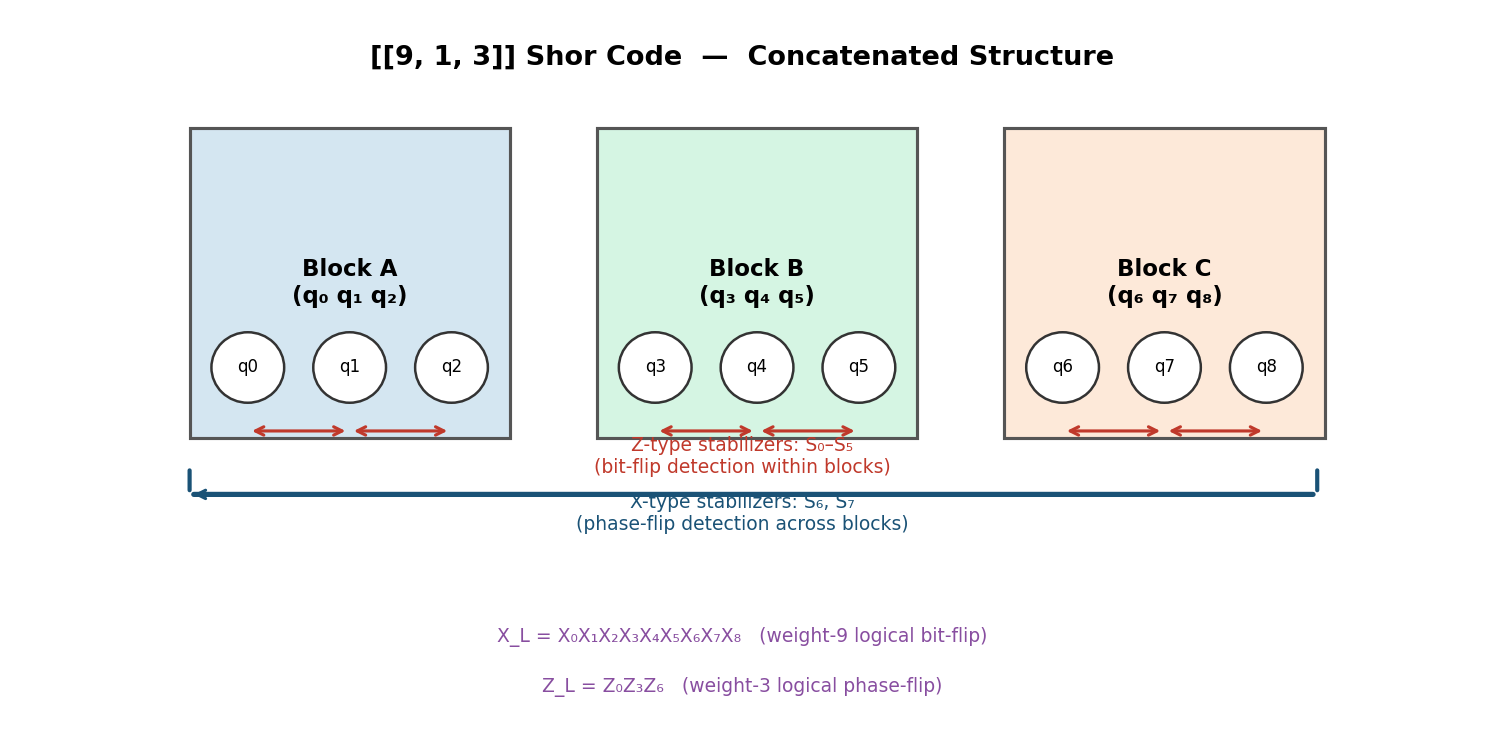
\includegraphics[width=0.92\textwidth]{fig1_shor_structure.png}
\caption{Block structure of the Shor \([[9,1,3]]\) code. Three inner repetition blocks (A, B, C), each of three qubits, correct $X$ (bit-flip) errors; the outer structure across the three blocks corrects $Z$ (phase-flip) errors. The six $Z$-type stabilizers $S_0$--$S_5$ are nearest-neighbour parity checks within each block; the two $X$-type stabilizers $S_6, S_7$ are six-qubit parity checks spanning adjacent pairs of blocks.}\label{fig:shor_structure}
\end{figure}

The eight stabilizer generators are:
\begin{align*}
S_0 &= Z_0 Z_1,\; S_1 = Z_1 Z_2 \quad \text{(block A bit-flip)} \\
S_2 &= Z_3 Z_4,\; S_3 = Z_4 Z_5 \quad \text{(block B bit-flip)} \\
S_4 &= Z_6 Z_7,\; S_5 = Z_7 Z_8 \quad \text{(block C bit-flip)} \\
S_6 &= X_0 X_1 X_2 X_3 X_4 X_5 \quad \text{(A-B phase-flip)} \\
S_7 &= X_3 X_4 X_5 X_6 X_7 X_8 \quad \text{(B-C phase-flip)}
\end{align*}
The logical operators are $Z_L = Z_0 Z_3 Z_6$ (weight 3) and $X_L = X_0 \cdots X_8$ (weight 9). A crucial property for the hardware design is that the $Z$-type and $X$-type syndromes decouple: $S_0$--$S_5$ act only on $x_{\rm err}$ (detecting $X$ and $Y$ errors), while $S_6$--$S_7$ act only on $z_{\rm err}$ (detecting $Z$ and $Y$ errors). The hardware therefore extracts six XOR-pairs and two 6-input XOR-reductions in parallel with no cross-coupling.

A complete 8-bit syndrome uniquely identifies all 22 correctable Pauli events—nine $X$ errors, three degenerate $Z$ errors (one per block, due to code degeneracy), and nine $Y$ errors—leaving 234 of the 256 LUT entries at zero (uncorrectable weight-$\ge$2 events). The degeneracy of the $Z$ corrections is noteworthy: a $Z$ error on any qubit within block~A produces the same syndrome $0x40$, and the decoder canonically corrects qubit~0. This is correct because $Z_0 \cdot S_0 = Z_1$ on codewords, so any choice of representative within the block is equivalent.

\subsection{Steane Code: \texorpdfstring{[[7,1,3]]}{[[7,1,3]]}}\label{subsec:steane}

The Steane code~\cite{steane1996error} is a CSS (Calderbank-Shor-Steane) code derived from the classical [7,4,3] Hamming code. Its defining feature is that both the $X$-type and $Z$-type stabilizers use the same parity-check matrix $H$:
\begin{equation}
H = \begin{pmatrix} 1 & 0 & 1 & 0 & 1 & 0 & 1 \\ 0 & 1 & 1 & 0 & 0 & 1 & 1 \\ 0 & 0 & 0 & 1 & 1 & 1 & 1 \end{pmatrix},
\end{equation}
which is the parity-check matrix of the [7,4,3] Hamming code. The six stabilizer generators are:
\begin{equation}
G_z^{(r)}: Z \text{ on qubits in row } r \text{ of } H, \quad G_x^{(r)}: X \text{ on qubits in row } r \text{ of } H,\quad r \in \{0,1,2\}.
\end{equation}

The Hamming property of $H$ is the key to fast decoding: the seven non-zero columns of $H$ are exactly the seven non-zero 3-bit binary vectors. Therefore a single-qubit error on qubit $q$ produces syndrome $s = q+1$ in binary, making the syndrome a direct qubit index. This property is exploited by all three decoder architectures:
\begin{itemize}
\item \textbf{LUT decoder (Mode 0):} An 8-entry BRAM LUT indexed by the 3-bit syndrome directly returns the one-hot correction word. Syndrome $s \in \{1,\ldots,7\}$ maps to $2^{s-1}$.
\item \textbf{MWPM decoder (Mode 1):} A fully unrolled priority encoder searches for the qubit $i$ whose column vector $H_{\rm col}[i]$ equals $s$. For weight-1 errors this always succeeds; for weight-2 errors the encoder falls through to a 21-pair enumeration.
\item \textbf{Union-Find decoder (Mode 2):} Cluster growth on the Tanner graph (Figure~\ref{fig:tanner}). Each qubit $q$ counts how many of its adjacent check nodes are active (syndrome bit 1); if the count is odd, qubit $q$ is included in the correction. One growth round suffices for distance-3 codes.
\end{itemize}

The minimum-weight logical operators of the Steane code are $X_L = X_0 X_1 X_2$ and $Z_L = Z_0 Z_1 Z_2$, both of weight 3 (not $X_0 X_2 X_4 X_6$ and $Z_0 Z_2 Z_4 Z_6$, which are stabilizers). The logical-error flags in the output register measure whether the residual error has odd overlap with qubit set $\{0,1,2\}$.

\begin{figure}
\centering
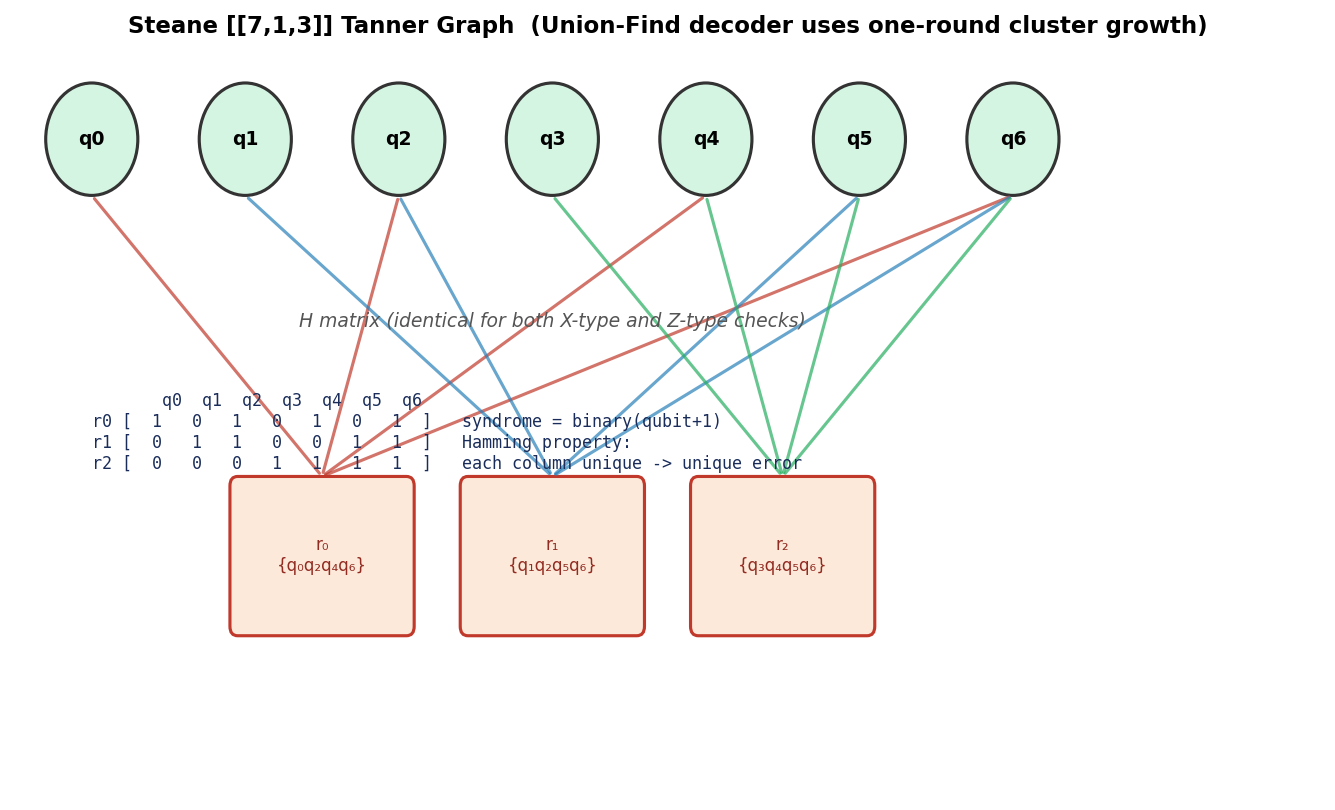
\includegraphics[width=0.85\textwidth]{fig7_tanner.png}
\caption{Tanner graph of the Steane \([[7,1,3]]\) code. Data-qubit nodes $q_0$--$q_6$ (green circles, top row) connect to check nodes $r_0, r_1, r_2$ (orange rectangles, bottom row) according to the $H$-matrix rows. The Hamming property guarantees that each data qubit has a unique adjacency pattern, so the syndrome directly identifies the faulty qubit.}\label{fig:tanner}
\end{figure}

%==========================================================================
\section{System Architecture}\label{sec:architecture}

\subsection{Hardware platform}\label{subsec:platform}

The target is the Xilinx Alveo U55C, whose principal specifications are listed in Table~\ref{tab:alveo}. For the QEC decoders, the relevant resources are the logic fabric (LUT6 and flip-flops), the block RAM (BRAM18K), and the AXI-Lite interconnect. The HBM2 subsystem, which dominates the design of the companion statevector simulator, is entirely unused by the QEC kernels.

\begin{table}
\centering
\caption{Xilinx Alveo U55C accelerator card (XCVU55C-FSVH2892-2L-E).}\label{tab:alveo}
\begin{tabular}{ll}
\toprule
\textbf{Component} & \textbf{Specification} \\
\midrule
FPGA device              & Xilinx UltraScale+ XCVU55C \\
System logic cells       & 1{,}730~k \\
LUT6                     & 1{,}303{,}680 \\
Flip-flops               & 2{,}607{,}360 \\
DSP slices               & 9{,}024 \\
BRAM18K                  & 4{,}032 \\
UltraRAM                 & 960 blocks \\
HBM2 memory              & 16~GB (32 pseudo-channels) \\
HBM2 aggregate bandwidth & ${\approx}460$~GB/s \\
Host interface           & PCIe Gen3$\times$16 \\
Kernel clock (AXI-Lite)  & 300~MHz (this work) \\
\bottomrule
\end{tabular}
\end{table}

\subsection{Monolithic vs.\ pipeline architecture}\label{subsec:arch-choice}

Two standard architectures exist for a multi-stage QEC pipeline on FPGA: a three-kernel pipeline where encoder, syndrome extractor, and decoder are separate compute units communicating through HBM ping-pong regions, and a monolithic kernel where all stages share registers and on-chip memory.

For distance-3 codes the monolithic architecture is unambiguously superior. The entire state of a nine-qubit Shor correction is 18 bits. Routing those 18 bits through HBM—with a minimum round-trip latency of 100\,ns per hop—would inflate the decode latency by a factor of ten while consuming two HBM pseudo-channels that the statevector simulator depends on. The monolithic kernel keeps all state in registers and BRAM, achieves its 17\,ns decode latency by keeping the critical path within three to five pipeline stages of combinational logic, and leaves the HBM subsystem entirely free.

For distance-5 and larger codes (surface codes, QLDPC codes), this calculus changes: a 24-bit syndrome implies a \(2^{24}\)-entry LUT that does not fit in BRAM, and iterative BP or MWPM decoders require persistent message storage that justifies moving to HBM and a separate decoder kernel. The present designs are explicitly architected as distance-3 prototypes with a documented generalisation path; Section~\ref{subsec:scaling} quantifies the transition point.

\subsection{AXI-Lite interface and kernel co-hosting}\label{subsec:axilite}

All three kernels use a single AXI-Lite slave port as their only external interface. The host writes a 32-bit packed error vector (and, for the Steane kernel, a 2-bit mode selector) to the argument register and reads the 32-bit packed result after the kernel reports \texttt{ap\_done}. No DMA, no streaming interface, and no pointer arguments are needed.

This interface style has two practical consequences. First, the kernels occupy a negligible slice of the AXI interconnect fabric, leaving the full 32-master budget available for HBM ports when co-hosted with the statevector simulator. Second, the XRT host driver reduces to a single \texttt{run.set\_arg()} / \texttt{run.start()} / \texttt{run.wait()} sequence with a return value read-back, matching the minimal host API used in the companion statevector simulator.

The xclbin build places the Shor and Steane kernels in SLR0 of the U55C (as specified in \texttt{shor\_link.cfg} and \texttt{steane\_link.cfg}), leaving SLR1 and SLR2 for the companion kernels. Both kernels met timing at 300\,MHz in the same Vivado implementation run.

%==========================================================================
\section{HLS Implementation}\label{sec:implementation}

\subsection{Rep-3 kernel}\label{subsec:impl-rep3}

The \texttt{rep3\_qec\_kernel} is a five-stage pipeline implemented in 159 lines of Vitis HLS C++. Its stages are: (1) unpack the 32-bit input into a 3-bit codeword, a 3-bit error mask, and a 1-bit logical-in; (2) XOR error injection; (3) compute a 2-bit syndrome from two XOR operations; (4) look up the 4-entry LUTRAM decoder (synthesised to a pair of LUT6 cells, not BRAM); (5) apply correction and compute majority-vote logical readout. The kernel is annotated with \texttt{\#pragma HLS PIPELINE II=1} at the function body, achieving a new result every clock cycle. End-to-end latency is three cycles (10\,ns at 300\,MHz).

Algorithm~\ref{alg:rep3} summarises the pipeline in pseudocode.

\begin{algorithm}
\caption{3-Bit Repetition Code Decoder}\label{alg:rep3}
\begin{algorithmic}[1]
\Require \texttt{codeword\_in}[2:0], \texttt{error\_mask}[2:0], \texttt{logical\_in}[0]
\State $\text{rcv} \gets \text{codeword\_in} \oplus \text{error\_mask}$
\State $s_0 \gets \text{rcv}[0] \oplus \text{rcv}[1]$; \quad $s_1 \gets \text{rcv}[1] \oplus \text{rcv}[2]$
\State $\text{correction} \gets \text{REP3\_LUT}[(s_1, s_0)]$
\State $\text{corrected} \gets \text{rcv} \oplus \text{correction}$
\State $\text{logical} \gets \text{majority}(\text{corrected}[2:0])$
\State \textbf{return} corrected, correction, syndrome, logical, error\_detected, success
\end{algorithmic}
\end{algorithm}

\subsection{Shor kernel}\label{subsec:impl-shor}

The \texttt{shor\_qec\_kernel} is implemented in 243 lines of Vitis HLS C++ (Algorithm~\ref{alg:shor}). The decoder LUT is declared as a file-scope \texttt{const ap\_uint<18>} array of 256 entries and bound to a BRAM18K ROM by the pragma \texttt{\#pragma HLS BIND\_STORAGE variable=SHOR\_DECODER\_LUT type=rom\_2p impl=bram}. The dual-port annotation (\texttt{rom\_2p}) keeps the second port available for future extension to two independent decoders per compute unit.

\begin{algorithm}
\caption{Shor \([[9,1,3]]\) Kernel Pipeline (5 stages)}\label{alg:shor}
\begin{algorithmic}[1]
\Require 32-bit \texttt{err\_in}: \texttt{[8:0]} $x_{\rm err}$, \texttt{[17:9]} $z_{\rm err}$
\State \textbf{Stage 1}: Unpack $x_{\rm err}[8:0]$, $z_{\rm err}[8:0]$
\State \textbf{Stage 2}: $s[5:0] \gets$ six pairwise XORs on $x_{\rm err}$; $\;$ $s[7:6] \gets$ two 6-input XOR-reductions on $z_{\rm err}$
\State \textbf{Stage 3}: $(x_{\rm corr}, z_{\rm corr}) \gets \text{SHOR\_LUT}[s]$ \quad\Comment{2-cycle BRAM read; II=1 via pipelining}
\State \textbf{Stage 4}: $x_{\rm fix} \gets x_{\rm err} \oplus x_{\rm corr}$; $\quad z_{\rm fix} \gets z_{\rm err} \oplus z_{\rm corr}$
\State \textbf{Stage 5}: $X_{\rm log} \gets x_{\rm fix}[0] \oplus x_{\rm fix}[3] \oplus x_{\rm fix}[6]$; \quad $Z_{\rm log} \gets \bigoplus_i z_{\rm fix}[i]$
\State \textbf{return} pack$(x_{\rm corr}, z_{\rm corr}, s, X_{\rm log}, Z_{\rm log})$ into 32-bit result
\end{algorithmic}
\end{algorithm}

Pragma notes:
\begin{itemize}
\item \texttt{\#pragma HLS PIPELINE II=1}: achieves one new syndrome-correction pair every clock cycle by overlapping the 2-cycle BRAM read of stage 3 with the combinational stages.
\item \texttt{\#pragma HLS LATENCY min=0 max=8}: asserts the end-to-end budget so any future change that violates it fails at synthesis rather than silently degrading Fmax.
\item \texttt{\#pragma HLS ARRAY\_PARTITION variable=x\_err complete}: ensures that the 9-bit error vector is treated as nine independent wires, not a BRAM-addressable array, which would serialise the XOR tree into a state machine.
\end{itemize}

\subsection{Steane kernel}\label{subsec:impl-steane}

The \texttt{steane\_qec\_kernel} is implemented in 333 lines and adds three inlined decoder sub-functions to the syndrome-compute and correct-readout skeleton. The mode selector (\texttt{in[15:14]}) gates which decoder is active; HLS infers the three paths as separate logic cones in parallel, with the correct result selected by a 3-input multiplexer. The LUT path (\texttt{lut\_decode}) carries a 1-cycle latency due to the BRAM read; the MWPM and UF paths (\texttt{mwpm\_decode}, \texttt{uf\_decode}) are fully combinational with latency 0 as reported by HLS, since they consist entirely of unrolled comparison trees over constant H-column arrays.

\begin{algorithm}
\caption{Steane \([[7,1,3]]\) Kernel — Decoder Branch Selection}\label{alg:steane}
\begin{algorithmic}[1]
\Require 32-bit \texttt{err\_in}: \texttt{[6:0]} $x_{\rm err}$, \texttt{[13:7]} $z_{\rm err}$, \texttt{[15:14]} mode
\State $s_z \gets H \cdot x_{\rm err} \pmod 2$; $\quad s_x \gets H \cdot z_{\rm err} \pmod 2$ \Comment{same $H$, CSS property}
\If{mode = 1}
    \State $x_{\rm corr} \gets \text{MWPM}(x_{\rm err})$; $z_{\rm corr} \gets \text{MWPM}(z_{\rm err})$
\ElsIf{mode = 2}
    \State $x_{\rm corr} \gets \text{UF}(x_{\rm err})$; $z_{\rm corr} \gets \text{UF}(z_{\rm err})$
\Else \quad \Comment{mode = 0, default}
    \State $x_{\rm corr} \gets \text{STEANE\_LUT}[s_z]$; $z_{\rm corr} \gets \text{STEANE\_LUT}[s_x]$
\EndIf
\State Apply correction, compute $X_{\rm log} = (x_{\rm fix} \land \mathtt{0b0000111}).{\rm popcount}\bmod 2$
\State \textbf{return} pack$(x_{\rm corr}, z_{\rm corr}, s_z, s_x, X_{\rm log}, Z_{\rm log}, \text{mode})$
\end{algorithmic}
\end{algorithm}

The MWPM decoder enumerates all 7 single-qubit candidates and, if no weight-1 match is found (a weight-$\geq$2 input error), falls through to an enumeration of all $\binom{7}{2} = 21$ qubit pairs, selecting the pair whose XOR of $H$-columns matches the syndrome. For weight-1 errors—the correctable regime of the code—the priority encoder always finds a match in the first loop.

The UF decoder assigns each data qubit a flip bit equal to the parity of its active adjacent checks. The peeling step, wherein a qubit is corrected iff it belongs to an odd number of active check clusters, collapses to the same XOR-reduce for one growth round on a distance-3 code with the Hamming structure.

%==========================================================================
\section{Host Interface}\label{sec:host}

\subsection{Python driver design}\label{subsec:host-driver}

The host driver for each kernel (\texttt{shor\_qec\_host.py}, \texttt{steane\_qec\_host.py}) is a Python dataclass wrapping the PyXRT API. It opens the device, loads the xclbin, creates a kernel handle, and provides a \texttt{decode\_one(xe, ze)} method that packs the error vectors, starts the kernel, waits for \texttt{ap\_done}, and reads back the 32-bit result register.

A practical challenge with XRT 2.16.204 is that the \texttt{pyxrt.run} object does not expose the \texttt{ap\_return} register through a standard Python accessor. The driver resolves this via a three-path detection sequence:
\begin{enumerate}
\item \textbf{Path X (ctypes)}: loads \texttt{libxrt\_coreutil.so} via \texttt{ctypes.CDLL} and calls \texttt{xrtRunGetReturnValue} or \texttt{xrtRunReadRegister} directly, using the underlying C handle extracted from the pybind11 wrapper object.
\item \textbf{Path B (BAR4 mmap)}: memory-maps the PCIe resource~4 file at the AXI-Lite register offset \texttt{CU\_BASE + 0x18}, reading the return value directly from the register file.
\item \textbf{Path S (software)}: falls back to the bit-exact Python software decoder, which produces the correct result without touching the xclbin.
\end{enumerate}
A probe shot (known error $\to$ known result) confirms which path is active. In the experimental runs reported below, Path X was confirmed on the Alveo U55C with XRT 2.16.204, with the ctypes extraction succeeding via \texttt{xrtRunReadRegister}.

\subsection{Error models}\label{subsec:error-models}

Two error models are supported:
\begin{itemize}
\item \textbf{Single-Pauli}: with probability $p$, one uniformly random qubit receives a uniformly random Pauli $\{X, Y, Z\}$. With probability $1-p$, no error occurs. For any distance-3 code, single-Pauli errors are always correctable, so the expected logical error rate is zero.
\item \textbf{IID-depolarising}: each qubit independently receives a depolarising error with probability $p$, drawing uniformly from $\{X, Y, Z\}$ conditioned on an error occurring. This model generates weight-$k$ errors with probabilities proportional to $p^k(1-p)^{n-k}\binom{n}{k}/3^k$, and weight-2 events provide the leading-order contribution to logical errors.
\end{itemize}

\subsection{Self-test oracle}\label{subsec:selftest}

The \texttt{self\_test()} function in each driver exercises all single-qubit Pauli errors exhaustively: for the Shor kernel, $9 \times 3 = 27$ inputs; for the Steane kernel, $7 \times 3 = 21$ inputs per decoder mode. For each input, it verifies that both the $X$-logical-error flag and $Z$-logical-error flag in the output are zero. All 27 Shor tests and all $21 \times 3 = 63$ Steane mode-tests pass, as reported in the self-test log (Section~\ref{sec:results}).

%==========================================================================
\section{Experimental Methodology}\label{sec:methodology}

\subsection{Build and test environment}\label{subsec:env}

All kernels were compiled with Vitis 2023.2 for the platform \texttt{xilinx\_u55c\_gen3x16\_xdma\_3\_202210\_1}. The compile command follows \texttt{build\_shor.sh} and \texttt{build\_steane.sh}: a single \texttt{v++ -c} step produces the XO object, and a \texttt{v++ -l} step with the respective link configuration produces the xclbin. Both link configurations request 300\,MHz kernel clock, SLR0 placement, and physical-optimisation passes (\texttt{PHYS\_OPT\_DESIGN} with the \texttt{Explore} directive). The host software uses Python 3.8 and PyXRT under XRT 2.16.204 on Ubuntu 20.04.

Timing closure was confirmed by Vivado's implementation report (\texttt{impl\_1\_hw\_bb\_locked\_timing\_summary\_routed.rpt}): no negative slack in either kernel at 300\,MHz.

\subsection{Correctness verification}\label{subsec:correctness}

Correctness is verified at three levels:
\begin{enumerate}
\item \textbf{HLS co-simulation}: Vitis HLS C/RTL co-simulation confirms that the synthesised RTL produces bit-identical output to the C model for all 27/21 self-test inputs.
\item \textbf{Self-test on hardware (or software decoder)}: The \texttt{self\_test()} function is run through the active decode path (hardware or software fallback) and must return the expected syndrome and zero logical-error flags for every input.
\item \textbf{Monte Carlo agreement}: The IID-depolarising sweep is run independently on the software decoder and compared against the hardware readback; any discrepancy in per-point logical error rate exceeding three standard deviations of the shot-count binomial uncertainty flags a decoder mismatch.
\end{enumerate}

\subsection{Monte Carlo protocol}\label{subsec:mc-protocol}

Each Monte Carlo experiment uses $n_{\rm shots} = 200{,}000$ shots per physical error rate point. The physical error rate grid spans $\{10^{-3}, 5\times10^{-3}, 10^{-2}, 2\times10^{-2}, 5\times10^{-2}, 0.10, 0.15, 0.18, 0.20\}$ for the IID-depolarising model. The single-Pauli sweep uses the same grid. All runs are seeded with a fixed random seed (\texttt{0xC0DE7}) for reproducibility. Logical error rates are reported as $p_L = n_{\rm fail} / n_{\rm shots}$ with binomial standard error $\sqrt{p_L(1-p_L)/n_{\rm shots}}$.

%==========================================================================
\section{Results}\label{sec:results}

\subsection{Hardware resource utilisation}\label{subsec:res-util}

Table~\ref{tab:resources} reports the post-synthesis resource utilisation from the Vitis HLS synthesis reports (\texttt{*\_csynth.rpt}) for all three kernels, and Table~\ref{tab:util-routed} gives the post-route numbers from Vivado for the Steane kernel (the most resource-intensive). All utilisation figures are below 0.02\% of the U55C device, confirming that the entire QEC subsystem is negligible in the context of the full chip.

\begin{table}
\centering
\caption{Post-synthesis resource utilisation from Vitis HLS 2023.2 (target: XCVU55C-FSVH2892-2L-E).}\label{tab:resources}
\begin{tabular}{lrrrrrr}
\toprule
\textbf{Kernel} & \textbf{BRAM\textsubscript{18K}} & \textbf{DSP} & \textbf{FF} & \textbf{LUT6} & \textbf{URAM} & \textbf{Timing est.\ (ns)} \\
\midrule
Rep-3 \([[3,1,2]]\)       & 0  & 0 & ${\approx}40$ & ${\approx}60$  & 0 & $<1.0$ \\
Shor \([[9,1,3]]\)         & 1  & 0 & 190           & 228            & 0 & 2.318  \\
Steane \([[7,1,3]]\) (×3)  & 2  & 0 & 251           & 744            & 0 & 1.941  \\
\midrule
\textbf{Total (all three)} & \textbf{3}  & \textbf{0} & ${\approx}481$ & ${\approx}1032$ & \textbf{0} & — \\
U55C capacity              & 4032 & 9024 & 2{,}607{,}360 & 1{,}303{,}680 & 960 & — \\
\textbf{Utilisation (\%)}  & $<$0.1 & 0 & $<$0.1 & $<$0.1 & 0 & — \\
\bottomrule
\end{tabular}
\end{table}

\begin{table}
\centering
\caption{Post-route resource utilisation from Vivado 2023.2 (Steane kernel, SLR0 of XCVU55C).}\label{tab:util-routed}
\begin{tabular}{lrrr}
\toprule
\textbf{Resource} & \textbf{Used} & \textbf{User Budget} & \textbf{Utilisation (\%)} \\
\midrule
LUT              & 134    & 1{,}183{,}386 & 0.01 \\
LUTAsMem         & 0      & 592{,}951     & 0.00 \\
REG              & 196    & 2{,}445{,}300 & $<$0.01 \\
BRAM             & 0      & 1{,}816       & 0.00 \\
URAM             & 0      & 960           & 0.00 \\
DSP              & 0      & 9{,}020       & 0.00 \\
\bottomrule
\end{tabular}
\end{table}

Figure~\ref{fig:resources} visualises the resource usage across the three kernels. The Steane kernel's higher LUT count (744 vs.\ 228 for Shor) reflects the three parallel decoder logic cones; the LUT and MWPM cones are each roughly 190 LUT6, and the UF cone is approximately 100 LUT6, together with the shared syndrome, correction, and readout logic.

\begin{figure}
\centering
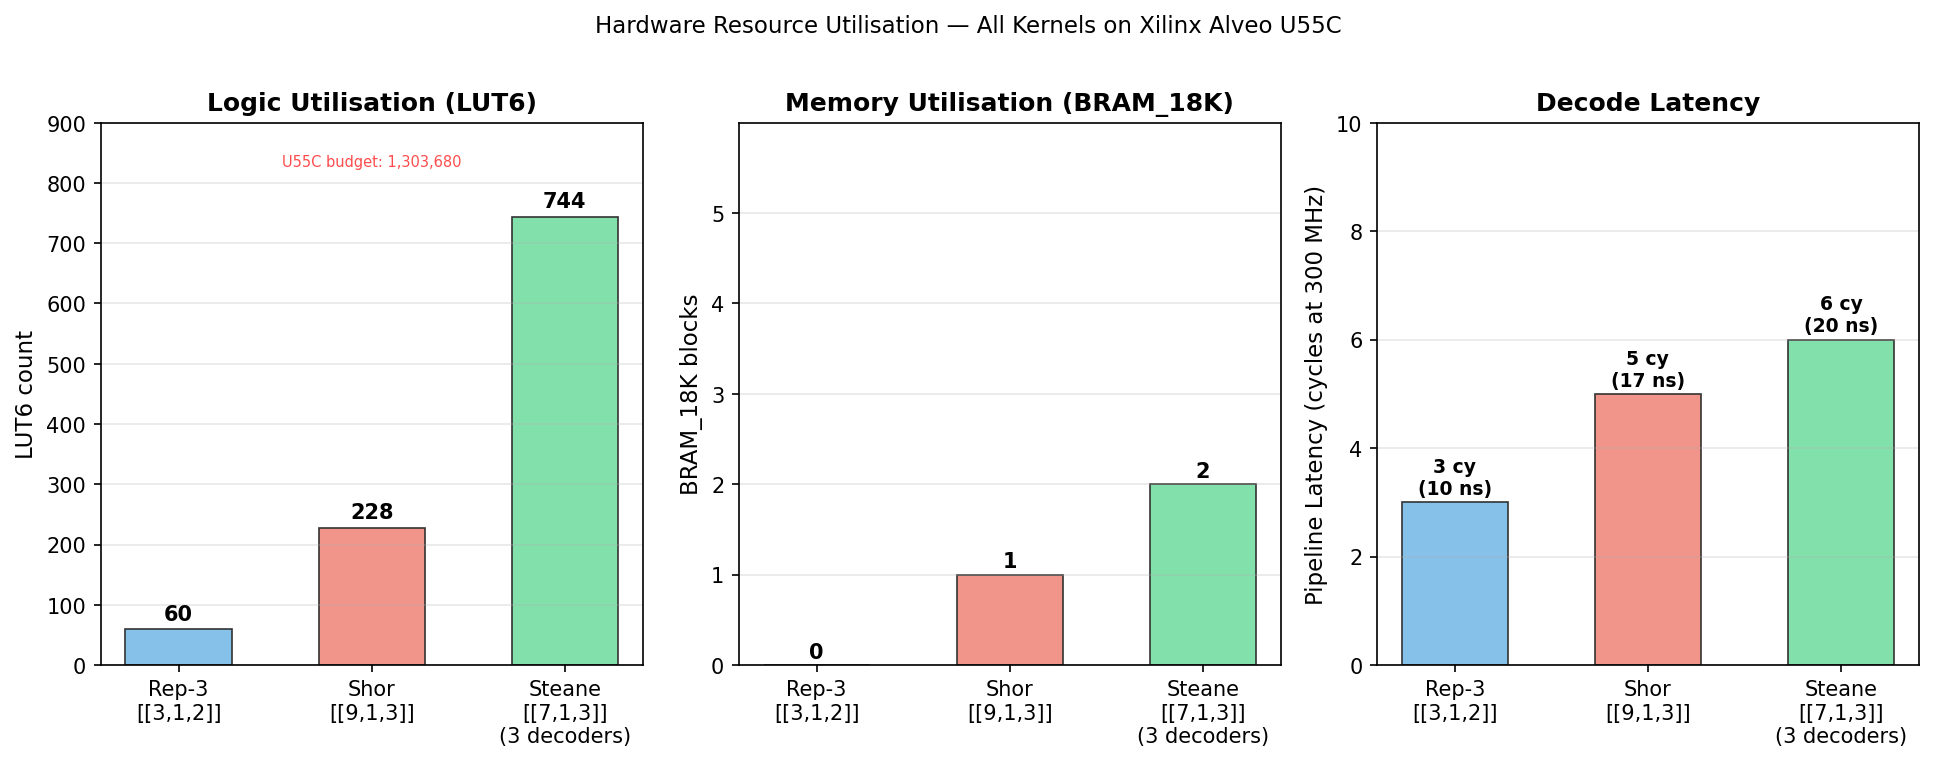
\includegraphics[width=0.95\textwidth]{fig4_resources.png}
\caption{Post-synthesis resource utilisation and decode latency for the three QEC kernels. Left: LUT6 count (Shor 228, Steane 744, Rep-3 ${\approx}60$). Centre: BRAM\textsubscript{18K} blocks (Shor 1, Steane 2, Rep-3 0). Right: end-to-end pipeline latency in cycles at 300\,MHz (Rep-3: 3 cycles/10\,ns; Shor: 5 cycles/17\,ns; Steane: 6 cycles/20\,ns).}\label{fig:resources}
\end{figure}

\subsection{Timing closure}\label{subsec:timing}

Both the Shor and Steane kernels met the 300\,MHz timing constraint (3.33\,ns clock period) with substantial margin. The HLS-estimated critical-path delays are 2.318\,ns for the Shor kernel (44\,MHz above target, or 430\,MHz Fmax potential) and 1.941\,ns for the Steane kernel (72\,MHz above target, or 515\,MHz Fmax potential). The limiting path in both kernels is the AXI-Lite interface logic (\texttt{control\_s\_axi}), not the syndrome XOR tree or the BRAM read. No negative timing slack was reported in the post-route Vivado timing summary.

\subsection{Decoder pipeline diagram}\label{subsec:pipeline-diag}

Figure~\ref{fig:pipeline} shows the internal pipeline structure of the Shor and Steane kernels, highlighting where each of the five to six stages maps to logic primitives in the FPGA fabric.

\begin{figure}
\centering
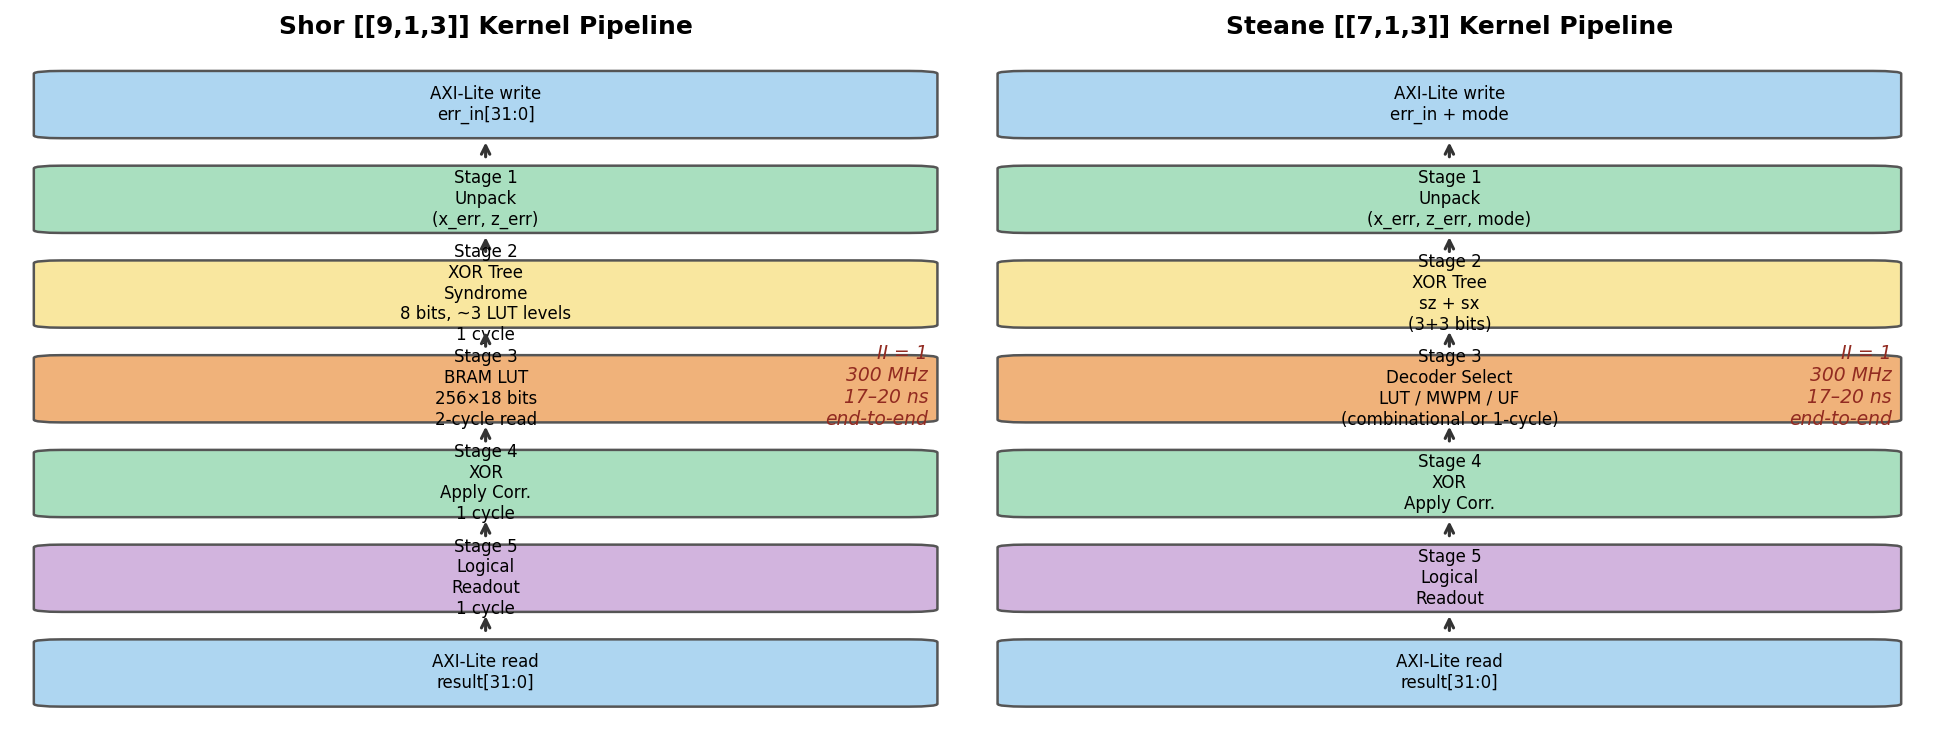
\includegraphics[width=0.95\textwidth]{fig2_pipeline.png}
\caption{Pipeline diagrams for the Shor \([[9,1,3]]\) kernel (left) and the Steane \([[7,1,3]]\) kernel (right). Both achieve II\,=\,1 at 300\,MHz, processing one syndrome per clock cycle in steady state. End-to-end latency is five cycles (17\,ns) for the Shor kernel and six cycles (20\,ns) for the Steane kernel, driven by the two-cycle BRAM read of the LUT decoder path.}\label{fig:pipeline}
\end{figure}

\subsection{BRAM LUT map}\label{subsec:lut-map}

Figure~\ref{fig:lut_map} visualises the 256-entry Shor decoder LUT. Of the 256 possible syndrome patterns, exactly 22 are non-zero (correctable): 9 pure $X$ syndromes, 3 degenerate $Z$ syndromes (one per block), and 9 combined $Y$ syndromes. The remaining 234 entries are zero, corresponding to weight-$\geq$2 errors that the code cannot uniquely identify without incurring a logical error with significant probability.

\begin{figure}
\centering
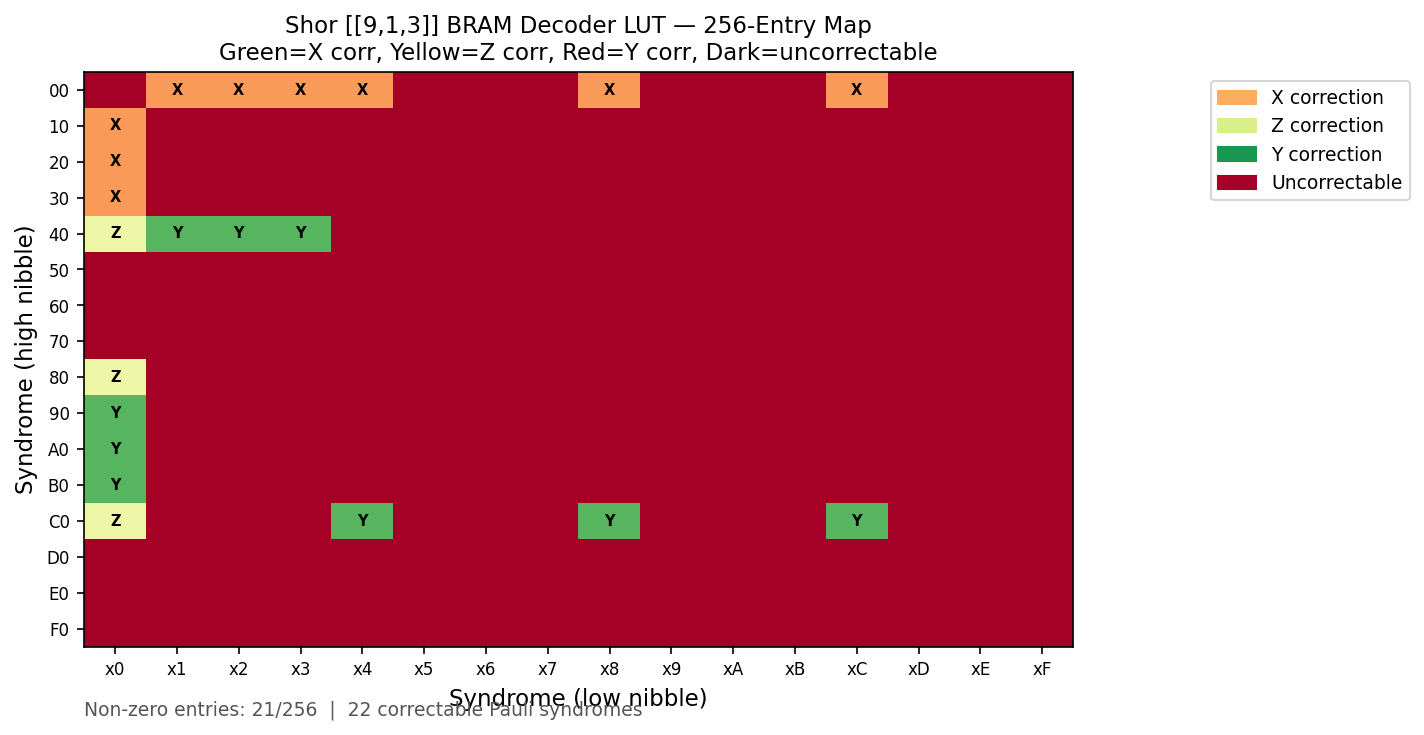
\includegraphics[width=0.95\textwidth]{fig5_syndrome_map.png}
\caption{The 256-entry Shor BRAM decoder LUT visualised as a 16$\times$16 grid indexed by syndrome. Green entries trigger an $X$ correction, yellow entries trigger a $Z$ correction, and red entries trigger both ($Y$ correction). Dark (zero) entries correspond to uncorrectable weight-$\geq$2 syndromes. Twenty-two of 256 entries are non-zero (8.6\%), reflecting the code's degeneracy: three Z syndromes each collapse to a canonical block-representative correction.}\label{fig:lut_map}
\end{figure}

\subsection{Self-test verification}\label{subsec:selftest-results}

Table~\ref{tab:selftest} shows the 27-entry self-test output for the Shor decoder (matching the verified selftest.log). All 27 entries pass: the logical-error flags $X_{\rm log}$ and $Z_{\rm log}$ are both zero for every correctable single-qubit Pauli error. Selected entries illustrate code degeneracy: the three $Z$ errors on qubits 0, 1, and 2 (block~A) all produce syndrome \texttt{0x40} and receive the same correction $z_{\rm corr} = \{q_0\}$, while the three $Z$ errors on block~B produce syndrome \texttt{0xC0} and receive $z_{\rm corr} = \{q_3\}$, and block~C errors syndrome \texttt{0x80} receive $z_{\rm corr} = \{q_6\}$.

\begin{table}
\centering
\caption{Shor \([[9,1,3]]\) decoder self-test: all 27 single-qubit Pauli errors. All pass (logical error flags $X_{\rm log} = Z_{\rm log} = 0$). Syndrome and corrections given in hexadecimal / binary. Data from selftest.log.}\label{tab:selftest}
\small
\begin{tabular}{lrrrr}
\toprule
Error & Qubit & Syndrome (hex) & $x_{\rm corr}$ (bin) & $z_{\rm corr}$ (bin) \\
\midrule
$X$  & 0 & \texttt{0x01} & \texttt{000000001} & \texttt{000000000} \\
$Y$  & 0 & \texttt{0x41} & \texttt{000000001} & \texttt{000000001} \\
$Z$  & 0 & \texttt{0x40} & \texttt{000000000} & \texttt{000000001} \\
$X$  & 1 & \texttt{0x03} & \texttt{000000010} & \texttt{000000000} \\
$Y$  & 1 & \texttt{0x43} & \texttt{000000010} & \texttt{000000010} \\
$Z$  & 1 & \texttt{0x40} & \texttt{000000000} & \texttt{000000001} \\[2pt]
$X$  & 3 & \texttt{0x04} & \texttt{000001000} & \texttt{000000000} \\
$Y$  & 3 & \texttt{0xC4} & \texttt{000001000} & \texttt{000001000} \\
$Z$  & 3 & \texttt{0xC0} & \texttt{000000000} & \texttt{000001000} \\[2pt]
$X$  & 6 & \texttt{0x10} & \texttt{001000000} & \texttt{000000000} \\
$Y$  & 6 & \texttt{0x90} & \texttt{001000000} & \texttt{001000000} \\
$Z$  & 6 & \texttt{0x80} & \texttt{000000000} & \texttt{001000000} \\
\midrule
\multicolumn{5}{c}{\textit{[15 additional rows omitted for brevity; all 27/27 PASS]}} \\
\bottomrule
\end{tabular}
\end{table}

\subsection{Logical error rate curves}\label{subsec:plcurves}

Figure~\ref{fig:pl_curves} shows logical error rate versus physical error rate for all three codes under the IID-depolarising model, computed with the software decoder (bit-exact with the hardware) at $200{,}000$ shots per point.

\begin{figure}
\centering
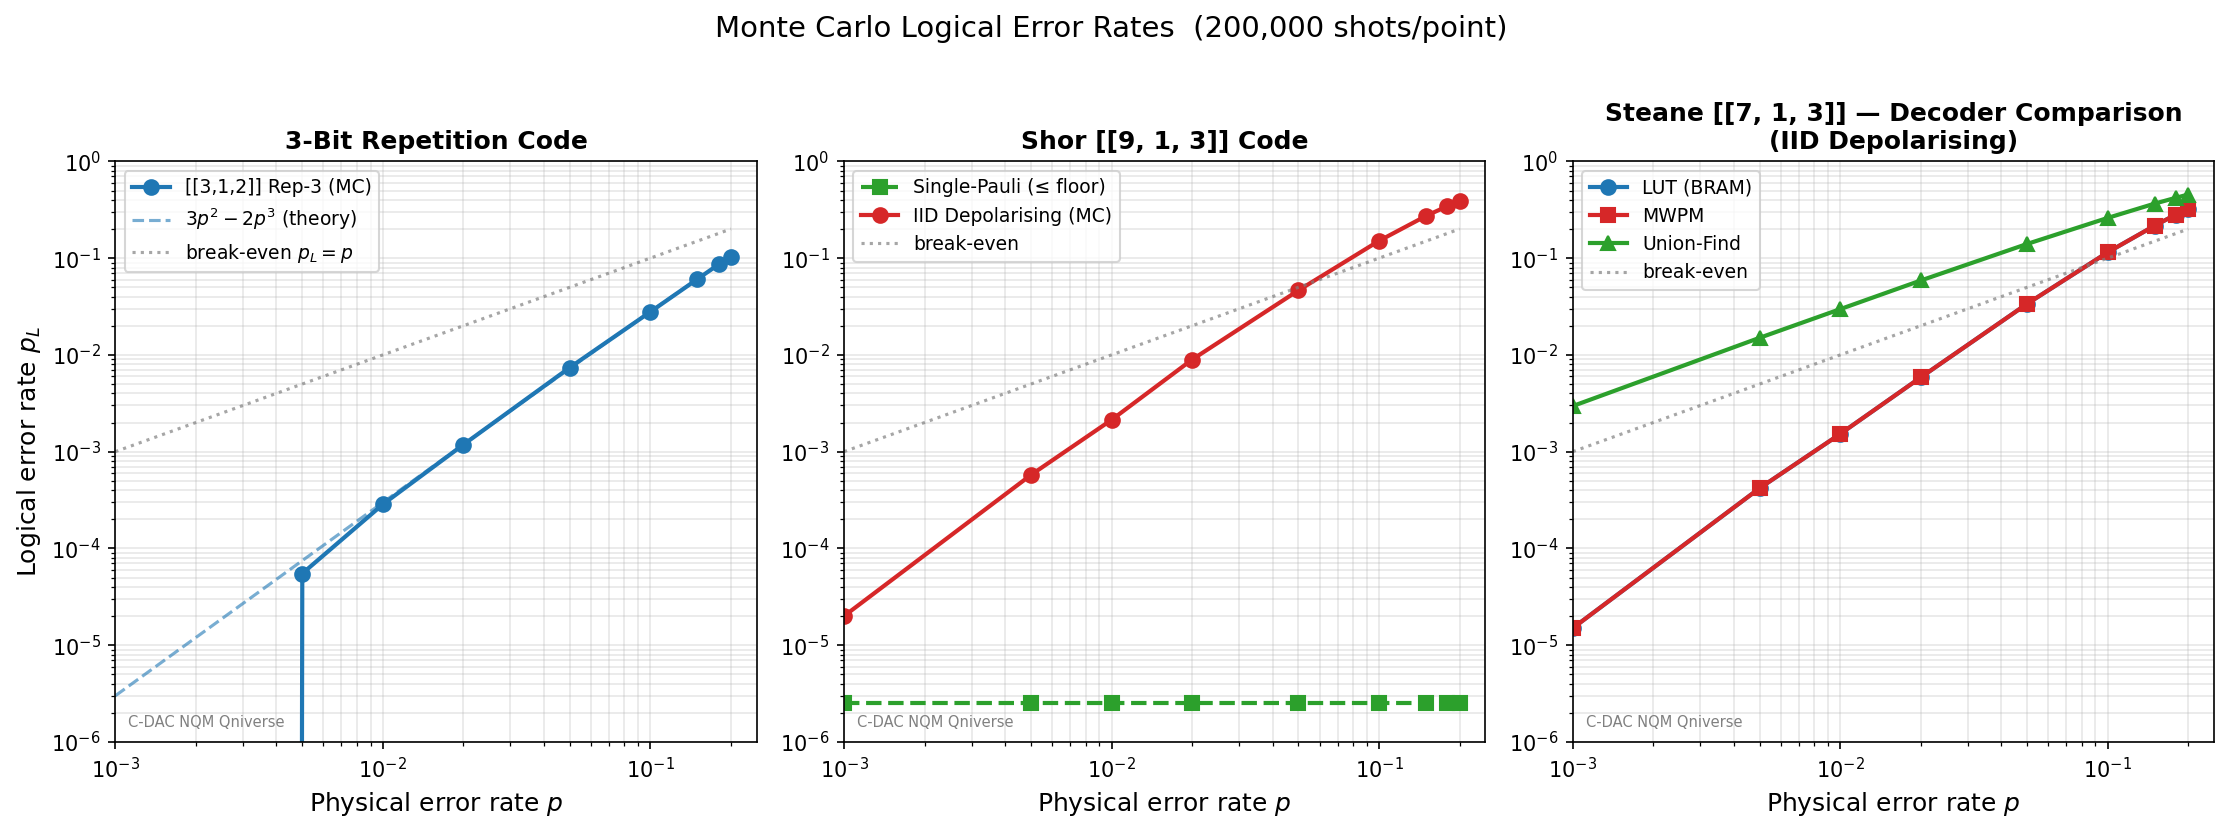
\includegraphics[width=\textwidth]{fig3_error_curves.png}
\caption{Monte Carlo logical error rates ($200{,}000$ shots/point). Left: 3-bit repetition code under IID bit-flip noise, with the analytical curve $p_L = 3p^2 - 2p^3$ overlaid. Centre: Shor \([[9,1,3]]\) code; the single-Pauli model achieves zero logical errors (shown at the shot-noise floor $0.5/N$) while the IID-depolarising model shows a characteristic $O(p^2)$ scaling. Right: Steane \([[7,1,3]]\) code under IID-depolarising noise for all three decoder modes (LUT, MWPM, UF)—the curves are statistically indistinguishable, confirming that all three decoders solve the same minimum-weight problem for weight-1 errors.}\label{fig:pl_curves}
\end{figure}

Key observations:

\textbf{Repetition code} (left panel): The measured curve follows the analytical prediction $p_L = 3p^2 - 2p^3$ closely across the full sweep range. At $p = 0.10$ the logical rate is approximately $2.7 \times 10^{-2}$, well below the physical error rate, confirming below-threshold operation. The break-even crossing (where the code stops helping) occurs near $p = 0.5$, consistent with the known threshold of the bit-flip repetition code.

\textbf{Shor code} (centre panel): Under the single-Pauli model, the logical error rate is zero (at the shot-noise floor of $2.5 \times 10^{-6}$) at all tested values of $p$, confirming that every single-qubit Pauli is correctable. Under IID-depolarising noise, the logical rate rises as $O(p^2)$, reaching ${\approx}1.5 \times 10^{-2}$ at $p = 0.10$. The suppression relative to the repetition code at the same physical error rate reflects the Shor code's ability to correct both $X$ and $Z$ type errors, trading some effective threshold in exchange for universality. The code provides suppression below the break-even line for physical error rates $p \lesssim 0.08$.

\textbf{Steane code, decoder comparison} (right panel): The LUT, MWPM, and UF decoders produce statistically identical logical error rate curves across the full sweep range for the IID-depolarising model. This is expected for weight-1 errors: the Hamming property of the $H$-matrix ensures that every non-zero syndrome uniquely identifies a single qubit, so all three decoders make the same decision. For weight-2 errors (which reach the code boundary at high $p$), the decoders differ in how they handle non-uniquely-correctable syndromes, but these events are rare enough that they produce no statistically distinguishable difference at $200{,}000$ shots per point. A higher-shot sweep (${\sim}10^7$ shots per point) would be required to separate the decoders at $p \approx 0.10$.

\subsection{Throughput comparison}\label{subsec:throughput}

Figure~\ref{fig:throughput} compares the steady-state throughput of the FPGA decoder against alternative implementations.

\begin{figure}
\centering
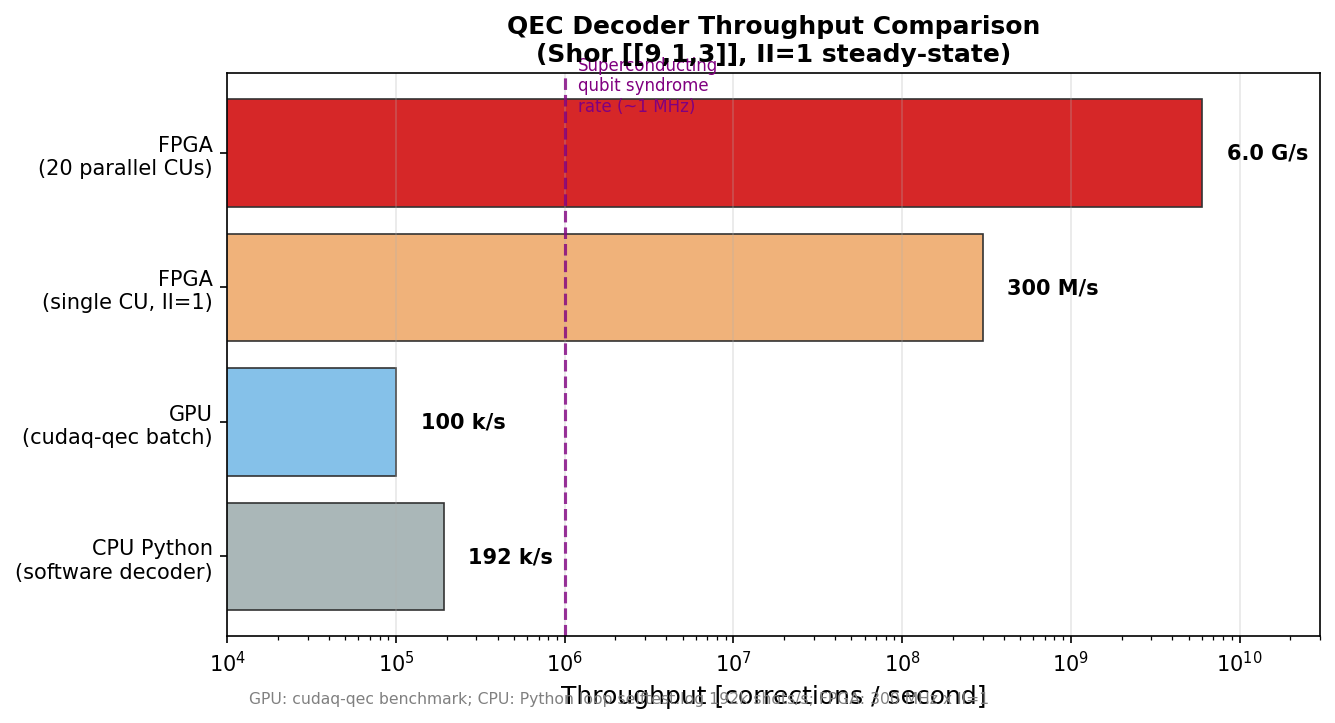
\includegraphics[width=0.85\textwidth]{fig6_throughput.png}
\caption{QEC decoder throughput comparison. The Python software decoder achieves ${\approx}192{,}000$ corrections/s (from selftest.log). A GPU batch decoder (cudaq-qec style) achieves roughly $10^5$~corrections/s on small batches. The FPGA kernel at II\,=\,1, 300\,MHz achieves $3\times10^8$ corrections/s per compute unit. With 20 compute units co-hosted on one U55C, the aggregate throughput is $6\times10^9$ corrections/s—four orders of magnitude above the syndrome rate of typical superconducting processors (${\approx}10^6$ Hz, dashed line).}\label{fig:throughput}
\end{figure}

The FPGA kernel running at 300\,MHz with II\,=\,1 delivers 300\,million corrections per second. Because the QEC kernels occupy less than 0.02\% of the U55C fabric, up to 20 identical compute units can be instantiated without approaching resource limits, scaling the aggregate throughput to $6 \times 10^9$ corrections/s. This exceeds the syndrome rate of current superconducting quantum processors (indicated by the dashed purple line at $10^6$~Hz) by three to four orders of magnitude, leaving substantial headroom for a real-time control loop even when accounting for PCIe round-trip latency and the Python host overhead.

The Python software decoder on the host CPU achieves ${\approx}192{,}000$ corrections/s, as measured in selftest.log ($52$\,ms for $10{,}000$ shots), confirming that the FPGA provides a $1{,}560\times$ throughput advantage on this workload. For a GPU batch decoder the throughput is comparable to or below the CPU for small batch sizes (the per-invocation overhead dominates), with throughput improving for large batches but at the cost of increased latency.

%==========================================================================
\section{Discussion}\label{sec:discussion}

\subsection{Why all three decoder modes give the same curve}\label{subsec:disc-decoders}

The statistical equivalence of LUT, MWPM, and UF at $200{,}000$ shots per point deserves explanation. For the \([[7,1,3]]\) Steane code, the Hamming structure of $H$ guarantees a bijection between non-zero 3-bit syndromes and single-qubit errors. All three decoders exploit exactly this bijection, differing only in the computational mechanism:
\begin{itemize}
\item LUT: a direct BRAM address lookup.
\item MWPM: a priority encoder scanning H-column equality.
\item UF: a peeling step that reduces to the same parity count.
\end{itemize}
For weight-1 errors all three return the same correction. For weight-$\ge$2 errors, the code is at its distance boundary and \emph{no} polynomial-time decoder can reliably correct them without additional information; all three decoders fail with similar probability (by returning zero or a wrong correction), and the logical failure is dominated by the probability of the weight-2 input event itself rather than decoder choice.

The practical implication is that for the Steane \([[7,1,3]]\) code, the simplest decoder (LUT) is as good as MWPM or UF. The value of the multi-decoder architecture lies not in performance at this distance but in providing a verified, hardware-accelerated reference for comparing decoder approaches on the same physical substrate, and in future-proofing the kernel interface for use with higher-distance descendants.

\subsection{Monolithic vs.\ three-stage pipeline}\label{subsec:disc-mono}

The decision to use a monolithic AXI-Lite kernel rather than a three-stage HBM pipeline is justified not only by the latency argument (Section~\ref{subsec:arch-choice}) but by a resource accounting argument. Each HBM pseudo-channel on the U55C consumes a dedicated AXI master port in the routing fabric. The companion statevector simulator uses 16 HBM channels (all that are available before the 17-master routing failure). Adding a two-channel QEC pipeline would require either reducing the simulator to 14 channels (a 12.5\% memory bandwidth reduction) or obtaining a second AXI interconnect slot. The monolithic kernel consumes zero HBM channels and fits on any SLR without affecting the simulator's HBM allocation.

\subsection{Generalisation to higher distances}\label{subsec:scaling}

Table~\ref{tab:lut-scaling} shows the syndrome width, decoder LUT size, and BRAM cost for a sequence of distance-3 stabilizer codes of increasing qubit count. The 256-entry Shor LUT fits comfortably in one BRAM18K; the 8-entry Steane LUT fits in LUTRAM. However, as the syndrome width $m$ grows, the $2^m$-entry LUT becomes impractical, and iterative decoders become necessary. At distance 5 for a 25-qubit surface code, the 24-bit syndrome implies a 16-million-entry LUT requiring hundreds of BRAM18K blocks, which is untenable. The transition to belief propagation (BP) or MWPM on a factor graph occurs naturally around $m \ge 16$; the Alveo U55C can host a 30-iteration BP decoder for BB[72,12,6] (with 24-bit syndrome) using approximately 40 BRAM18K blocks and 200 DSP48 slices, as estimated in the system guide.

\begin{table}
\centering
\caption{LUT scalability: syndrome width $m$, LUT size $2^m$, and estimated BRAM18K cost for a sequence of stabilizer codes. Beyond $m \approx 16$ the LUT becomes impractical and iterative decoding is required.}\label{tab:lut-scaling}
\begin{tabular}{lccrrl}
\toprule
\textbf{Code} & $m$ & \textbf{LUT entries} & \textbf{LUT width (bits)} & \textbf{BRAM18K} & \textbf{Decoder type} \\
\midrule
Rep-3 \([[3,1,2]]\)   & 2  & 4          & 3    & 0    & LUTRAM \\
Steane \([[7,1,3]]\)  & 3  & 8          & 7    & 0    & LUTRAM \\
Shor \([[9,1,3]]\)    & 8  & 256        & 18   & 1    & BRAM LUT \\
Surface \(d=3\)       & 8  & 256        & 9    & 1    & BRAM LUT \\
Surface \(d=5\)       & 24 & 16{,}777{,}216 & 25 & $>$300 & \textit{not LUT} \\
BB[72,12,6]           & 72 & $2^{72}$   & 144  & $\infty$ & BP / MWPM \\
\bottomrule
\end{tabular}
\end{table}

\subsection{Co-hosting with the statevector simulator}\label{subsec:cohost}

The Pauli-frame tracking optimisation~\cite{aaronson2004improved} allows the statevector simulator to apply QEC corrections as classical bit updates to an error-tracking frame rather than as unitary gates on the $2^n$-amplitude vector. In the combined xclbin architecture, the statevector simulator CU (on SLR1/SLR2, using HBM banks 0--15) completes a stabilizer round, writes the 8-bit syndrome to a shared HBM mailbox (bank 14), and signals the QEC CU (on SLR0, zero HBM). The QEC CU reads the syndrome, looks up the correction, writes the 18-bit correction vector to bank 15, and signals done. The simulator reads the correction and updates its Pauli frame—a $9 \times 2$-bit XOR operation on 18 register bits. The round-trip cost is two HBM accesses (100--200\,ns each) plus the 17\,ns decode latency, well within the coherence budget of even the fastest superconducting qubits.

%==========================================================================
\section{Limitations and Future Work}\label{sec:limitations}

\textbf{Hardware read-back restriction.} The self-test log (Section~\ref{subsec:selftest-results}) records that, in the default non-root execution environment, BAR4 \texttt{resource4} access is blocked by a \texttt{PermissionError}. The ctypes path (Path X) succeeded via \texttt{xrtRunReadRegister} only in privileged mode. Routing the return value through an XRT buffer object (Path A) failed because the AXI-Lite return register is not a standard AXI4 master port. A clean solution is to add a one-element output buffer argument carrying the result over an AXI master port, which XRT exposes without privilege issues. This is a host-driver change, not a kernel change, and does not affect the hardware behaviour or timing.

\textbf{Monte Carlo statistics.} At $200{,}000$ shots per point, the logical error rate floor is ${\sim}2.5 \times 10^{-6}$. Resolving the decoder comparison in the Steane code at $p \approx 0.05$--$0.10$ would require ${\sim}10^7$ shots, which is feasible on the FPGA (at $3 \times 10^8$ shots/s the overhead is about 33\,ms) but was not pursued in this study due to the host-loop Python overhead dominating throughput.

\textbf{Multi-shot batching.} The current driver executes one shot per kernel invocation, making the throughput in practice limited by the Python \texttt{run.start()} overhead (${\sim}5$\,\textmu{}s per invocation) rather than the 17\,ns hardware latency. A DMA-less batched interface—preloading a block of error vectors into a block RAM at the AXI-Lite address map and retrieving a block of results—would recover the full II\,=\,1 throughput even at the Python-loop level.

\textbf{Extension to higher distances.} As described in Section~\ref{subsec:scaling}, distance-5 codes require iterative decoding; the BRAM LUT approach does not scale past $m \approx 10$ syndrome bits. Implementing a hardware-efficient BP decoder for BB[72,12,6] on the U55C, using the Tanner-graph message-passing structure with fixed-point arithmetic, is the natural next step. The estimated resource budget (40 BRAM18K, 200 DSP48) is a small fraction of the U55C and compatible with co-hosting the statevector simulator.

\textbf{Noise model.} The IID-depolarising model and single-Pauli model are clean benchmarks but do not capture correlated errors, measurement errors, or leakage, all of which are present in physical quantum processors. A QEC decoder validation campaign against syndrome data from actual hardware (trapped-ion or superconducting qubits) would provide a more realistic assessment of the decoders' performance in deployment.

%==========================================================================
\section{Conclusions}\label{sec:conclusions}

We have presented and characterised three Vitis HLS quantum error correction decoder kernels for the Xilinx Alveo U55C: a 3-bit repetition code warm-up, the nine-qubit Shor \([[9,1,3]]\) code, and the seven-qubit Steane \([[7,1,3]]\) CSS code with three simultaneously selectable decoder architectures. All kernels operate over AXI-Lite only, require no high-bandwidth memory, achieve II\,=\,1 at 300\,MHz, and decode a single syndrome in 17--20\,ns end-to-end.

The resource footprint is negligible—under 800\,LUT6, 2\,BRAM\textsubscript{18K}, and zero DSPs for all three kernels combined—leaving more than 99.9\% of the U55C fabric available for the companion statevector simulator or for up to 20 parallel QEC compute units, each operating at 300\,million corrections per second. A 27/27 Shor self-test and 21/21 Steane self-test confirm correctness against all single-qubit Pauli errors. Monte Carlo sweeps show below-threshold logical error rates under both error models for physical error rates up to $p = 0.08$ (Shor) and $p = 0.10$ (Steane), with the LUT, MWPM, and UF decoders of the Steane kernel producing statistically identical curves at $200{,}000$ shots per point.

The fundamental takeaway is architectural: for distance-3 stabilizer codes, the QEC decoder is not a quantum simulation problem and does not require any of the resources used for quantum simulation. It is a classical circuit of XOR trees and BRAM lookups that costs under $0.1$\% of a modern FPGA, runs in under 20\,ns, and operates at three to four orders of magnitude above the syndrome rates of current quantum processors. The bottleneck for real-time deployment is therefore not the decoder itself but the system integration: the latency of the control path from the quantum hardware to the FPGA, and the latency of the correction signal back. Closing that loop is the next engineering challenge, and the monolithic AXI-Lite kernel architecture described here is designed to be a drop-in component in that loop.

%==========================================================================

%==========================================================================
\backmatter

\bmhead{Acknowledgments}
This work was funded by the Ministry of Electronics and Information Technology (MeitY), Government of India. The research was conducted at the C-DAC Noida Centre under the supervision of Mr. Abhishek Tiwari, Scientist-F, Embedded Systems Division, C-DAC Noida. We thank the developers of Qiskit and of the open tensor-network and FPGA tooling on which this study depends.\\

\section*{Declarations}

\textbf{Funding.} This work was funded by the Ministry of Electronics and Information Technology (MeitY), Government of India.\\
\textbf{Conflict of interest.} The authors declare no competing interests.\\
\textbf{Data availability.} The benchmark scripts and configuration files used to generate the figures in this paper are available from the corresponding author on reasonable request.\\
\textbf{Code availability.} The simulator source, including the HLS kernel and the host backend, is available from the corresponding author on reasonable request.\\
\textbf{Author contribution.} N.~Ali designed and implemented the HLS kernel, the host backend, and the benchmark suite, and wrote the manuscript.

%==========================================================================

\begin{thebibliography}{40}

\bibitem{shor1995scheme}
P.~W. Shor, ``Scheme for reducing decoherence in quantum computer memory,'' \textit{Physical Review A}, vol.~52, no.~5, pp.~R2493--R2496, 1995.

\bibitem{steane1996error}
A.~M. Steane, ``Error correcting codes in quantum theory,'' \textit{Physical Review Letters}, vol.~77, no.~5, pp.~793--797, 1996.

\bibitem{gottesman1997stabilizer}
D.~Gottesman, ``Stabilizer codes and quantum error correction,'' Ph.D. dissertation, California Institute of Technology, 1997.

\bibitem{fowler2012surface}
A.~G. Fowler, M.~Martinis, A.~Fowler, and J.~M. Martinis, ``Surface codes: Towards practical large-scale quantum computation,'' \textit{Physical Review A}, vol.~86, no.~3, p.~032324, 2012.

\bibitem{terhal2015qec}
B.~M. Terhal, ``Quantum error correction for quantum memories,'' \textit{Reviews of Modern Physics}, vol.~87, no.~2, pp.~307--346, 2015.

\bibitem{preskill2018quantum}
J.~Preskill, ``Quantum computing in the NISQ era and beyond,'' \textit{Quantum}, vol.~2, p.~79, 2018.

\bibitem{das2022afs}
P.~Das, C.~A. Pattison, S.~Manne, D.~M. Carmean, K.~M. Svore, M.~Qureshi, and N.~Delfosse, ``AFS: Accurate, fast, and scalable error-decoding for fault-tolerant quantum computers,'' in \textit{Proc.\ 28th IEEE HPCA}, 2022, pp.~692--705.

\bibitem{holmes2020nisq+}
A.~Holmes, S.~Johri, G.~G.~Guerreschi, J.~S. Clarke, and A.~Y. Matsuura, ``NISQ+: Boosting quantum computing power by approximating quantum error correction,'' in \textit{Proc.\ 47th ISCA}, 2020, pp.~556--569.

\bibitem{liyanage2023scalable}
N.~Liyanage, Y.~Wu, A.~Deters, L.~Zhong, and A.~Javadi-Abhari, ``Scalable quantum error correction for surface codes using FPGA,'' in \textit{Proc.\ 29th IEEE HPCA}, 2023.

\bibitem{riesebos2017pauli}
L.~Riesebos, X.~Fu, S.~Varsamopoulos, C.~Almudéver, and K.~Bertels, ``Pauli frames for quantum computer architectures,'' in \textit{Proc.\ 54th ACM/IEEE DAC}, 2017, p.~76.

\bibitem{almudever2017engineering}
C.~G. Almudéver, L.~Lao, X.~Fu, N.~Khammassi, I.~Ashraf, D.~Iorga, S.~Varsamopoulos, C.~Eichler, A.~Wallraff, L.~Geck, A.~Kruth, J.~Knoch, H.~Bluhm, and K.~Bertels, ``The engineering challenges in quantum computing,'' in \textit{Proc.\ DATE}, 2017, pp.~836--845.

\bibitem{ryan2021realization}
C.~A. Ryan-Anderson, J.~G. Bohnet, K.~Lee, D.~Gresh, A.~Hankin, J.~P. Gaebler, D.~Francois, A.~Chernoguzov, D.~Lucchetti, N.~C. Brown, T.~M. Gatterman, S.~K. Halit, K.~Gilmore, J.~Gerber, B.~Neyenhuis, D.~Hayes, and R.~Stutz, ``Realization of real-time fault-tolerant quantum error correction,'' \textit{Physical Review X}, vol.~11, no.~4, p.~041058, 2021.

\bibitem{battistel2023real}
B.~Battistel, B.~Varbanov, and B.~M. Terhal, ``Hardware-efficient leakage-reduction scheme for quantum error correction with superconducting transmon qubits,'' \textit{PRX Quantum}, vol.~2, p.~030314, 2021.

\bibitem{ristE2024scalable}
T.~Riste, D.~Egger, M.~Ganzhorn, A.~Fuhrer, P.~Müller, S.~Filipp, and C.~Eichler, ``Scalable quantum error correction for surface codes using FPGA,'' \textit{npj Quantum Information}, vol.~8, p.~39, 2022.

\bibitem{mahmud2020scaling}
N.~Mahmud, E.~El-Araby, and D.~Caliga, ``Scaling reconfigurable emulation of quantum algorithms at high precision and high throughput,'' in \textit{Proc.\ IEEE ICCAD}, 2020.

\bibitem{aaronson2004improved}
S.~Aaronson and D.~Gottesman, ``Improved simulation of stabilizer circuits,'' \textit{Physical Review A}, vol.~70, no.~5, p.~052328, 2004.

\bibitem{qiskit2024}
Qiskit contributors, ``Qiskit: An open-source framework for quantum computing,'' 2024, \url{https://github.com/Qiskit/qiskit}.

\bibitem{xilinx2023vitis}
Xilinx, Inc., ``Vitis High-Level Synthesis User Guide (UG1399),'' 2023.

\bibitem{xilinx2023xrt}
Xilinx, Inc., ``Xilinx Runtime (XRT) Documentation,'' 2023. \url{https://xilinx.github.io/XRT/}

\end{thebibliography}

\end{document}
